\documentclass{article}
\usepackage{CJK}
\usepackage{amsmath}
\usepackage{amsthm}
\usepackage{amsfonts}
\usepackage{palatino}
\usepackage{xcolor}
\usepackage{geometry}
\usepackage{listings}
\usepackage{pxfonts}
\usepackage{enumerate}
\usepackage[pdftex]{graphicx}
\geometry{left=2cm,right=2cm,top=3cm,bottom=3cm}
\pagestyle{myheadings}
\markright{Huiqian Yu/14300180118}
\setlength{\parindent}{0pt}
\newcommand{\ix}[1]{\intertext{{}#1}}
\newcommand{\dx}{\;\mathrm{d}\,x}
\newcommand{\dt}{\;\mathrm{d}\,t}
\newcommand{\dm}[1]{\;\mathrm{d}\,{}#1}
\newcommand{\ve}{\varepsilon}
\newcommand{\tp}{^\mathsf{T}}
\newcommand{\var}{\mathrm{var}}
\newcommand{\corr}{\mathrm{corr}}
\newcommand{\mbe}[1]{\mathbb{E}\left[{}#1\right]}
\newcommand{\argmin}[1]{\mathop{\arg\min}_{{}#1}}
\newcommand{\suml}[3]{\sum\limits_{#1=#2}^{#3}}
\begin{document}
\definecolor{backcolour}{rgb}{0.95,0.95,0.92}
\begin{CJK*}{GBK}{song}

\begin{enumerate}
\item[3.28]
	\begin{align*}
		\ix{For IMA(1, 1) model}
		x_{t}&=x_{t-1}+w_{t}-\lambda w_{t-1}
		\ix{Assume $y_{t}=w_{t}-\lambda w_{t-1}$, $y_{t}$ is invertible, and}
		x_{t}&=x_{t-1}+y_t\\
		y_{t}&=\suml j1\infty \lambda^{j}y_{t-j}+w_t\\
		x_t-x_{t-1}&=\suml j1\infty \lambda^{j}(x_{t-j}-x_{t-j-1})+w_t\\
		x_t  	&=\suml j1\infty \lambda^{j-1}(1-\lambda)x_{t-j}+w_t
	\end{align*}
\item[3.29]
	(a).\begin{align*}
		(1-\phi B)y_t&=\delta+w_t
		\ix{assume $z_t = y_t - \mu ,\mu=\dfrac{\delta}{1-\phi}$,}
		(1-\phi B)z_t&=w_t		
		\ix{in AR(1) model, $z_{n+j}^n$ is only related to $z_n$}
		z_{n+j}^n&=\phi^j z_n\\\tag{i}
		y_{n+j}^n&=\phi^j y_n + \dfrac{\delta(1-\phi^j)}{1-\phi}\\
				&=\phi^j y_n + \delta[1+\phi+\cdots+\phi^{j-1}]
	\ix{(b).From (i),}
		x_{n+m}^n-x_{n+m-1}^n=y_{n+m}^n&=\phi^j y_n + \dfrac{\delta(1-\phi^m)}{1-\phi}\\
		&=\phi^m (x_n-x_{n-1}) + \dfrac{\delta(1-\phi^m)}{1-\phi}\\
		x_{n+m}^n-x_n&=\suml k1m \phi^k(x_n-x_{n-1})+\suml k1m \dfrac{\delta(1-\phi^k)}{1-\phi}\\
		x_{n+m}^n&=x_n+(x_n-x_{n-1})\dfrac{\phi(1-\phi^m)}{1-\phi}+\delta\left[m-\dfrac{\phi(1-\phi^m)}{1-\phi}\right]
	\ix{(c)}
		\theta(z)&=1-\phi z\\
		\phi(z)&=z\\
		\psi^*(z)&=\phi(z)/\theta(z)(1-z)\\
				&=\dfrac{z}{(1-z)(1-\phi z)}\\
				&=z+(1+\phi)z+\cdots+\suml k1n \phi^{k-1}z^n\\
		P_{n+m}^n&=\sigma_w^2\suml j0{m-1}\psi_j^{*2}\\
				&=\sigma_w^2\suml j0{m-1}(\suml k1j \phi^{k-1})^2\\
				&=\sigma_w^2\suml j0{m-1}\dfrac{(1-\phi^{j+1})^2}{(1-\phi)^2}
	\end{align*}
\item[4.1]
	(a).\begin{center}
	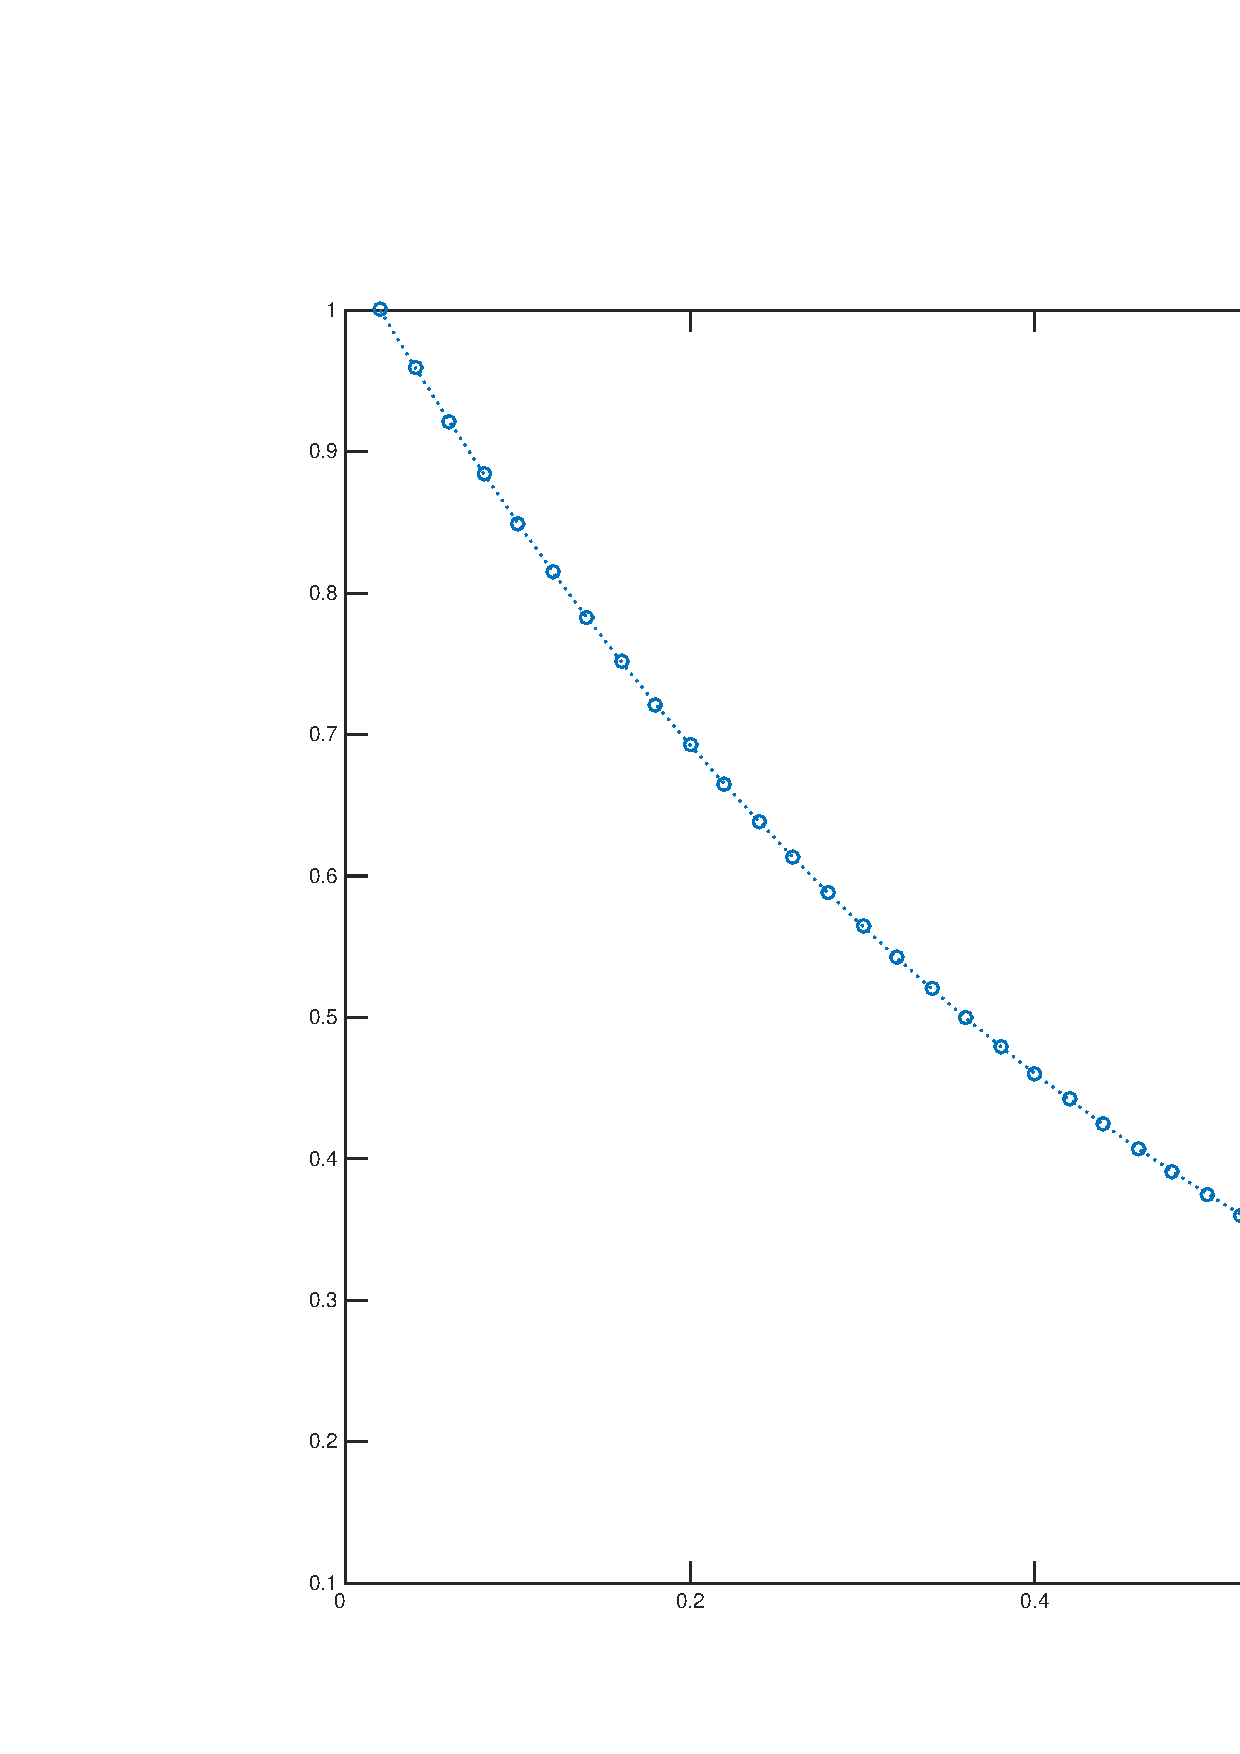
\includegraphics[width=12cm]{1.png}
	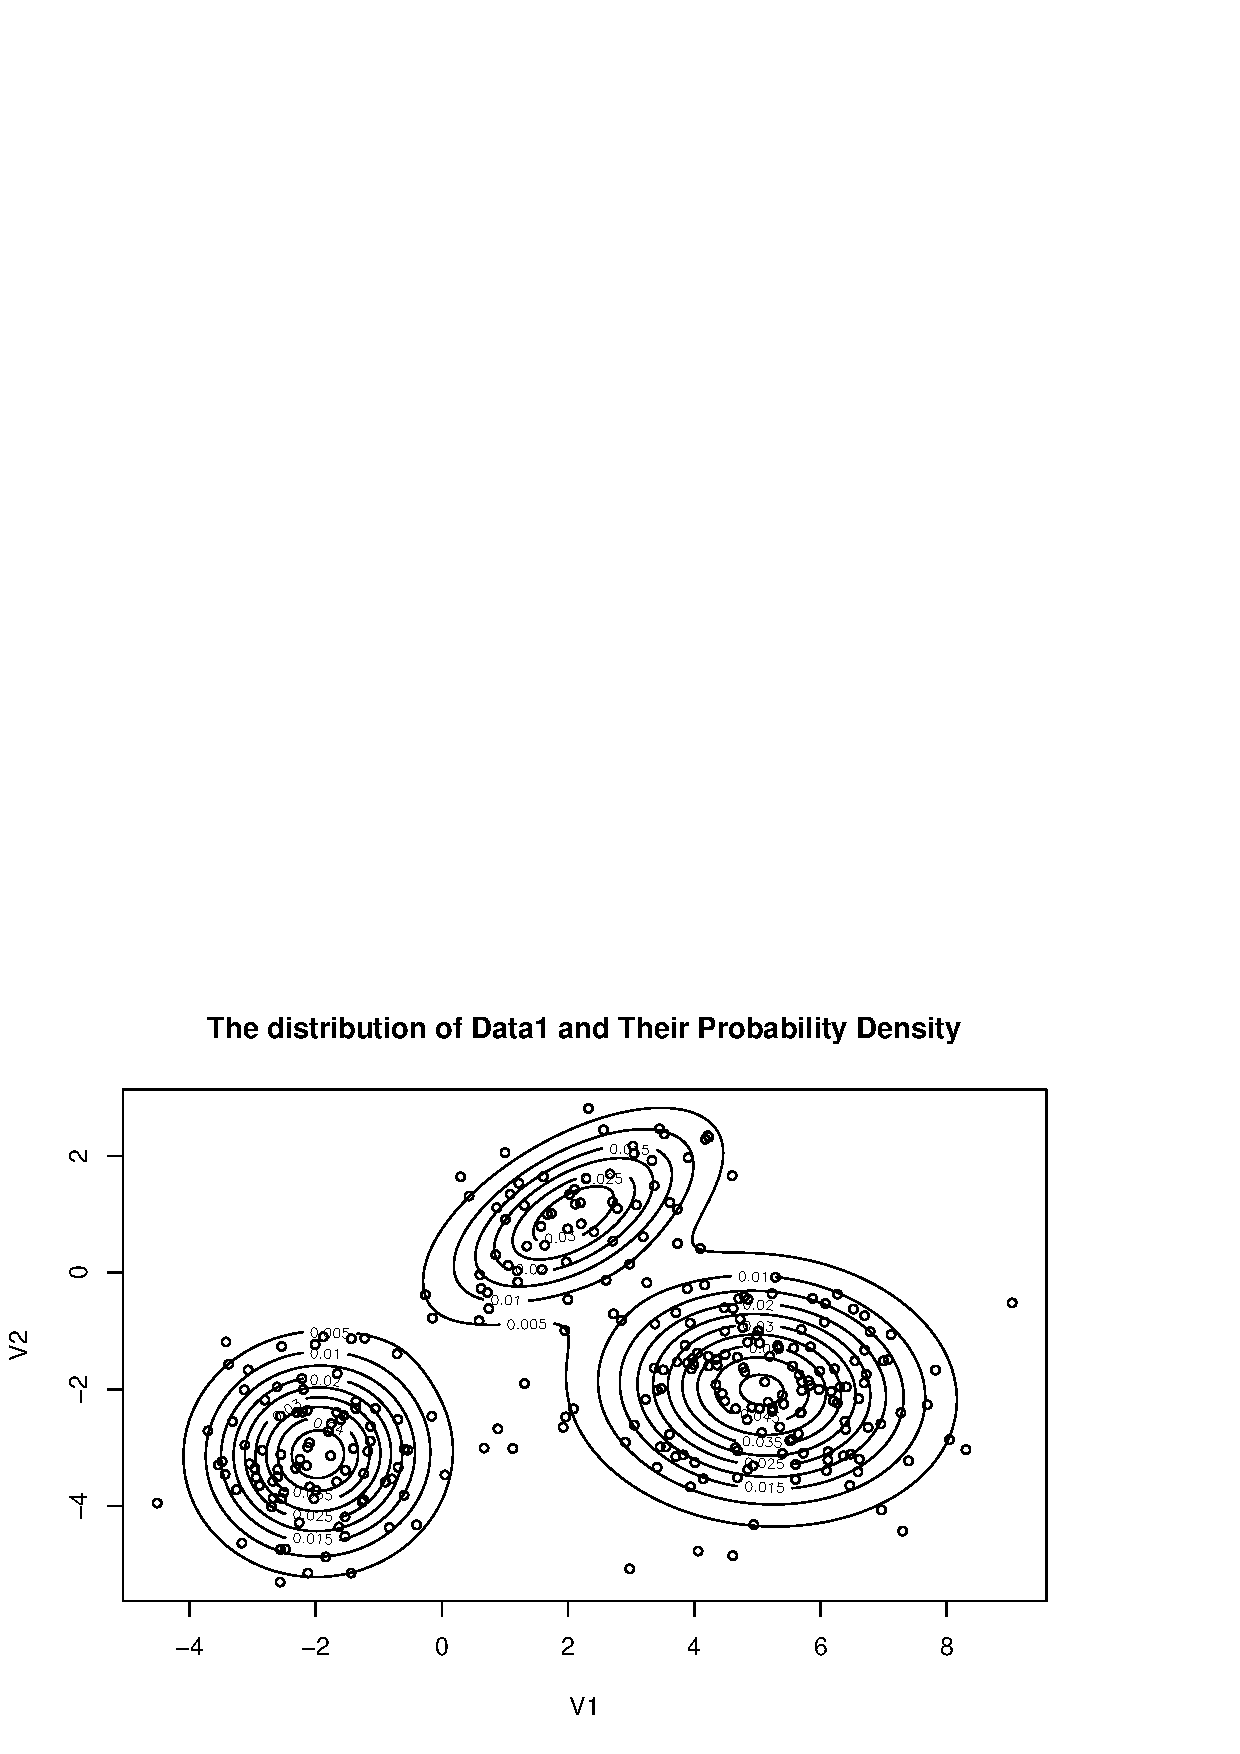
\includegraphics[width=12cm]{2.png}
	\end{center}
	The major difference between these series is that there is two completed peroid in the plot of sum.\\
	(b).\begin{center}
	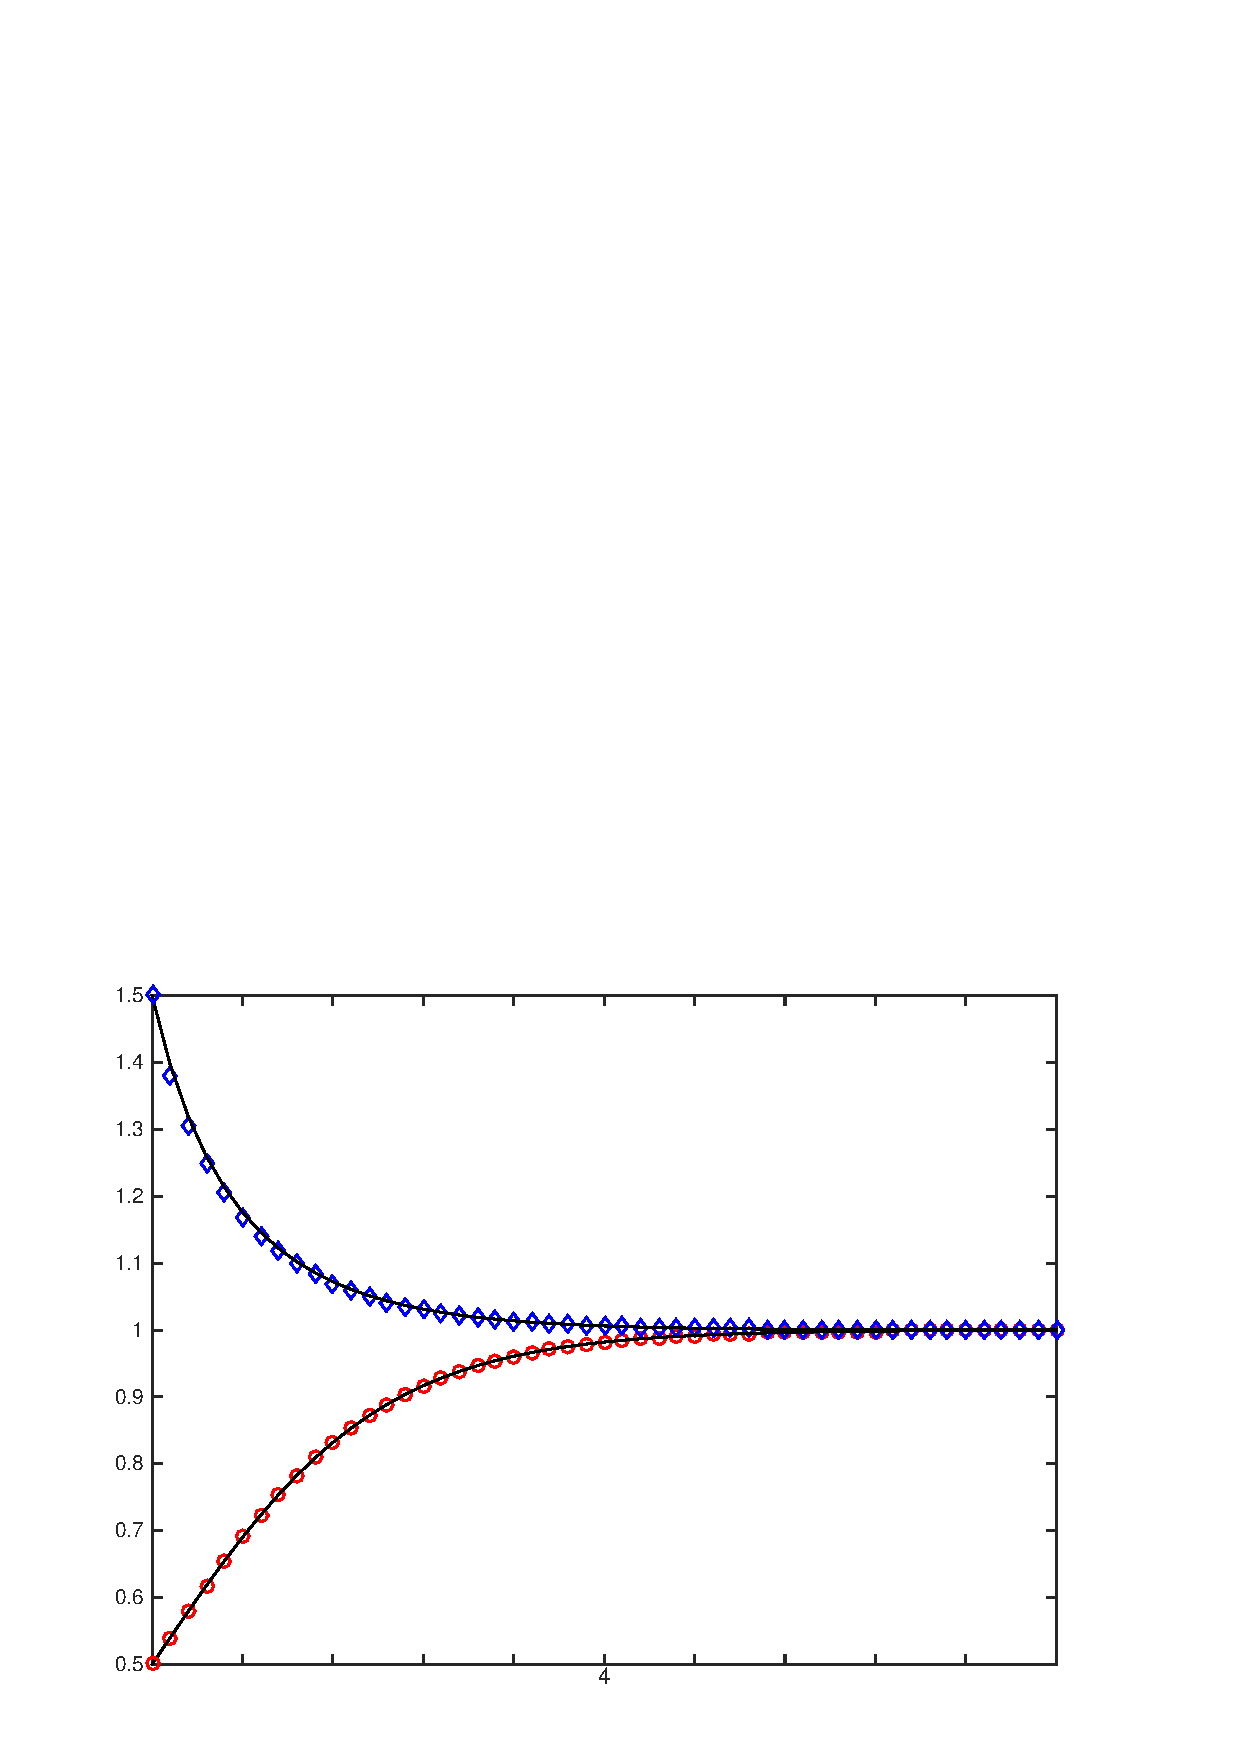
\includegraphics[width=8cm]{3.png}
	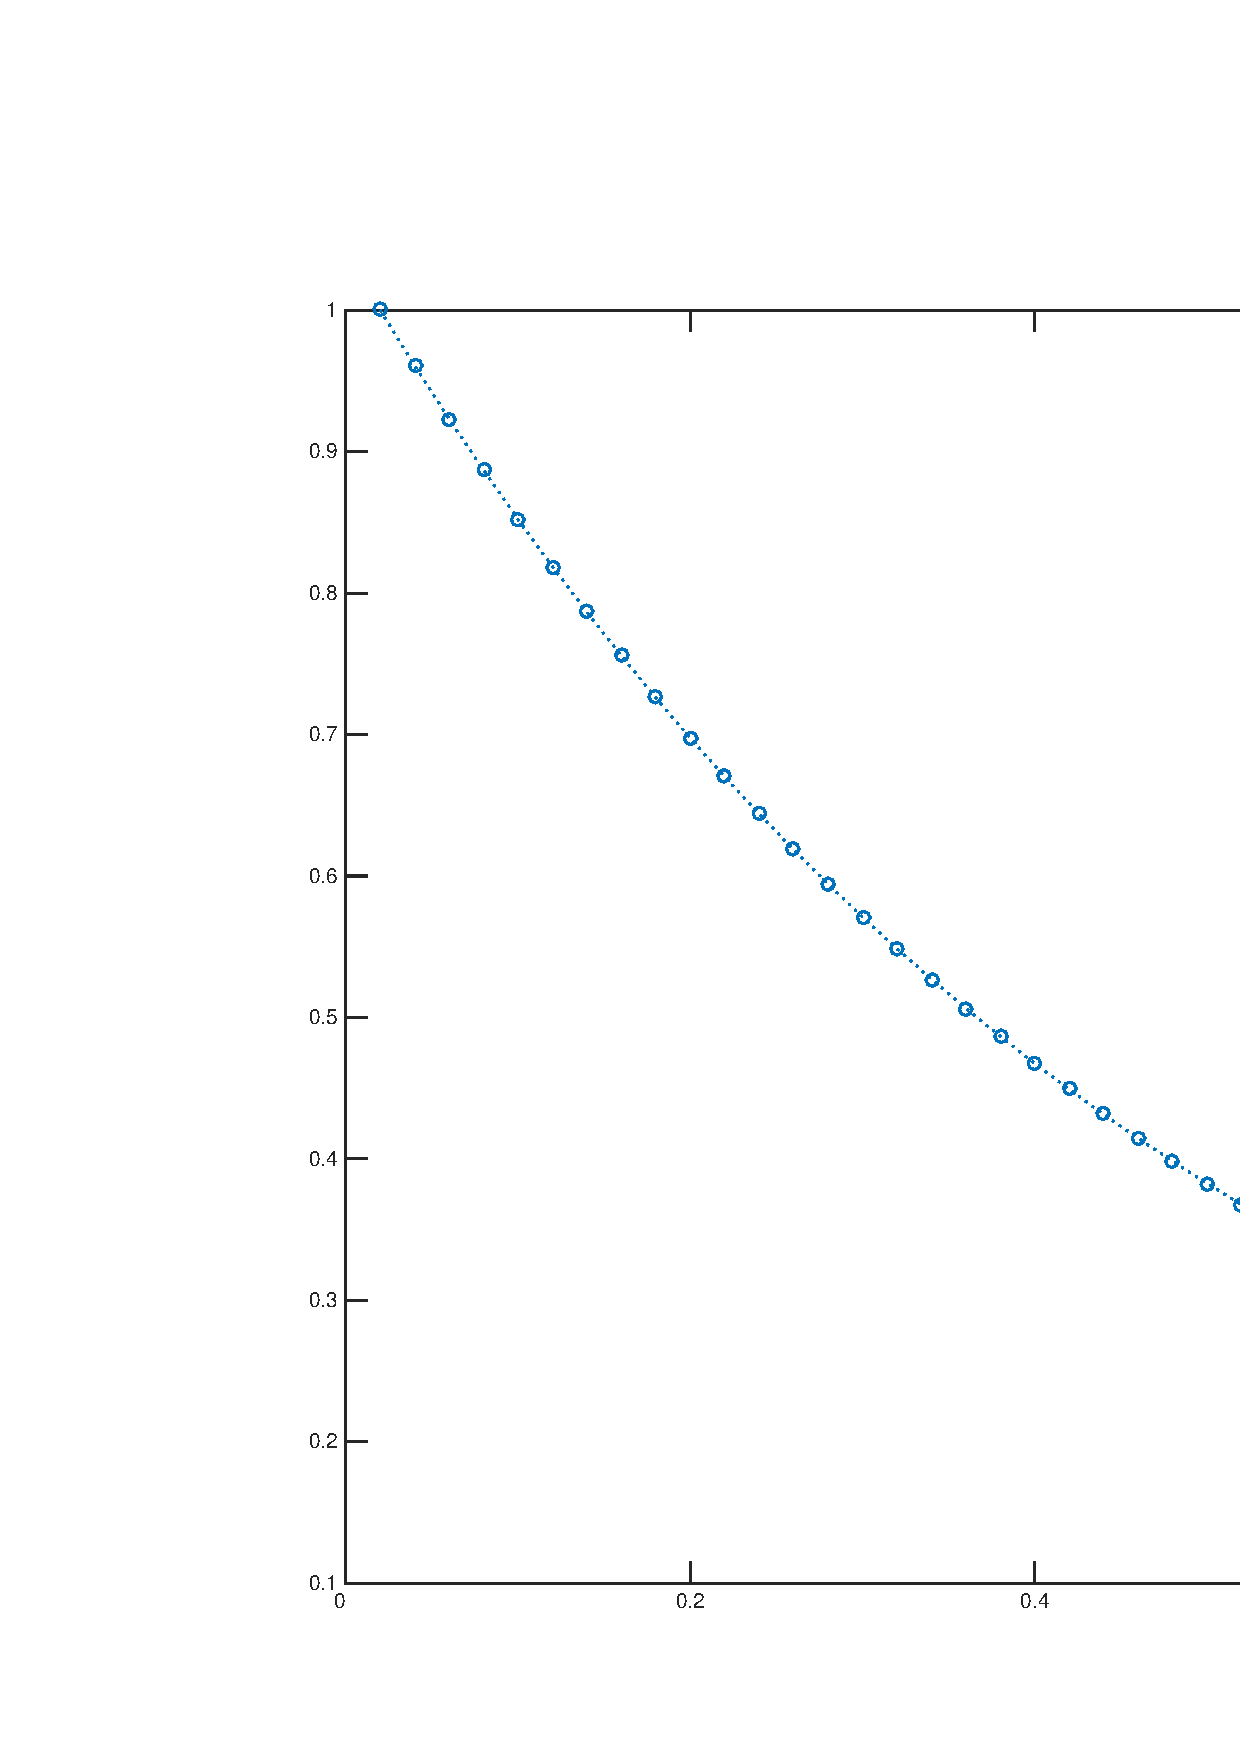
\includegraphics[width=8cm]{4.png}
	\end{center}
	The periodogram becomes larger with the change of $n$.\\
	(c).\begin{center}
	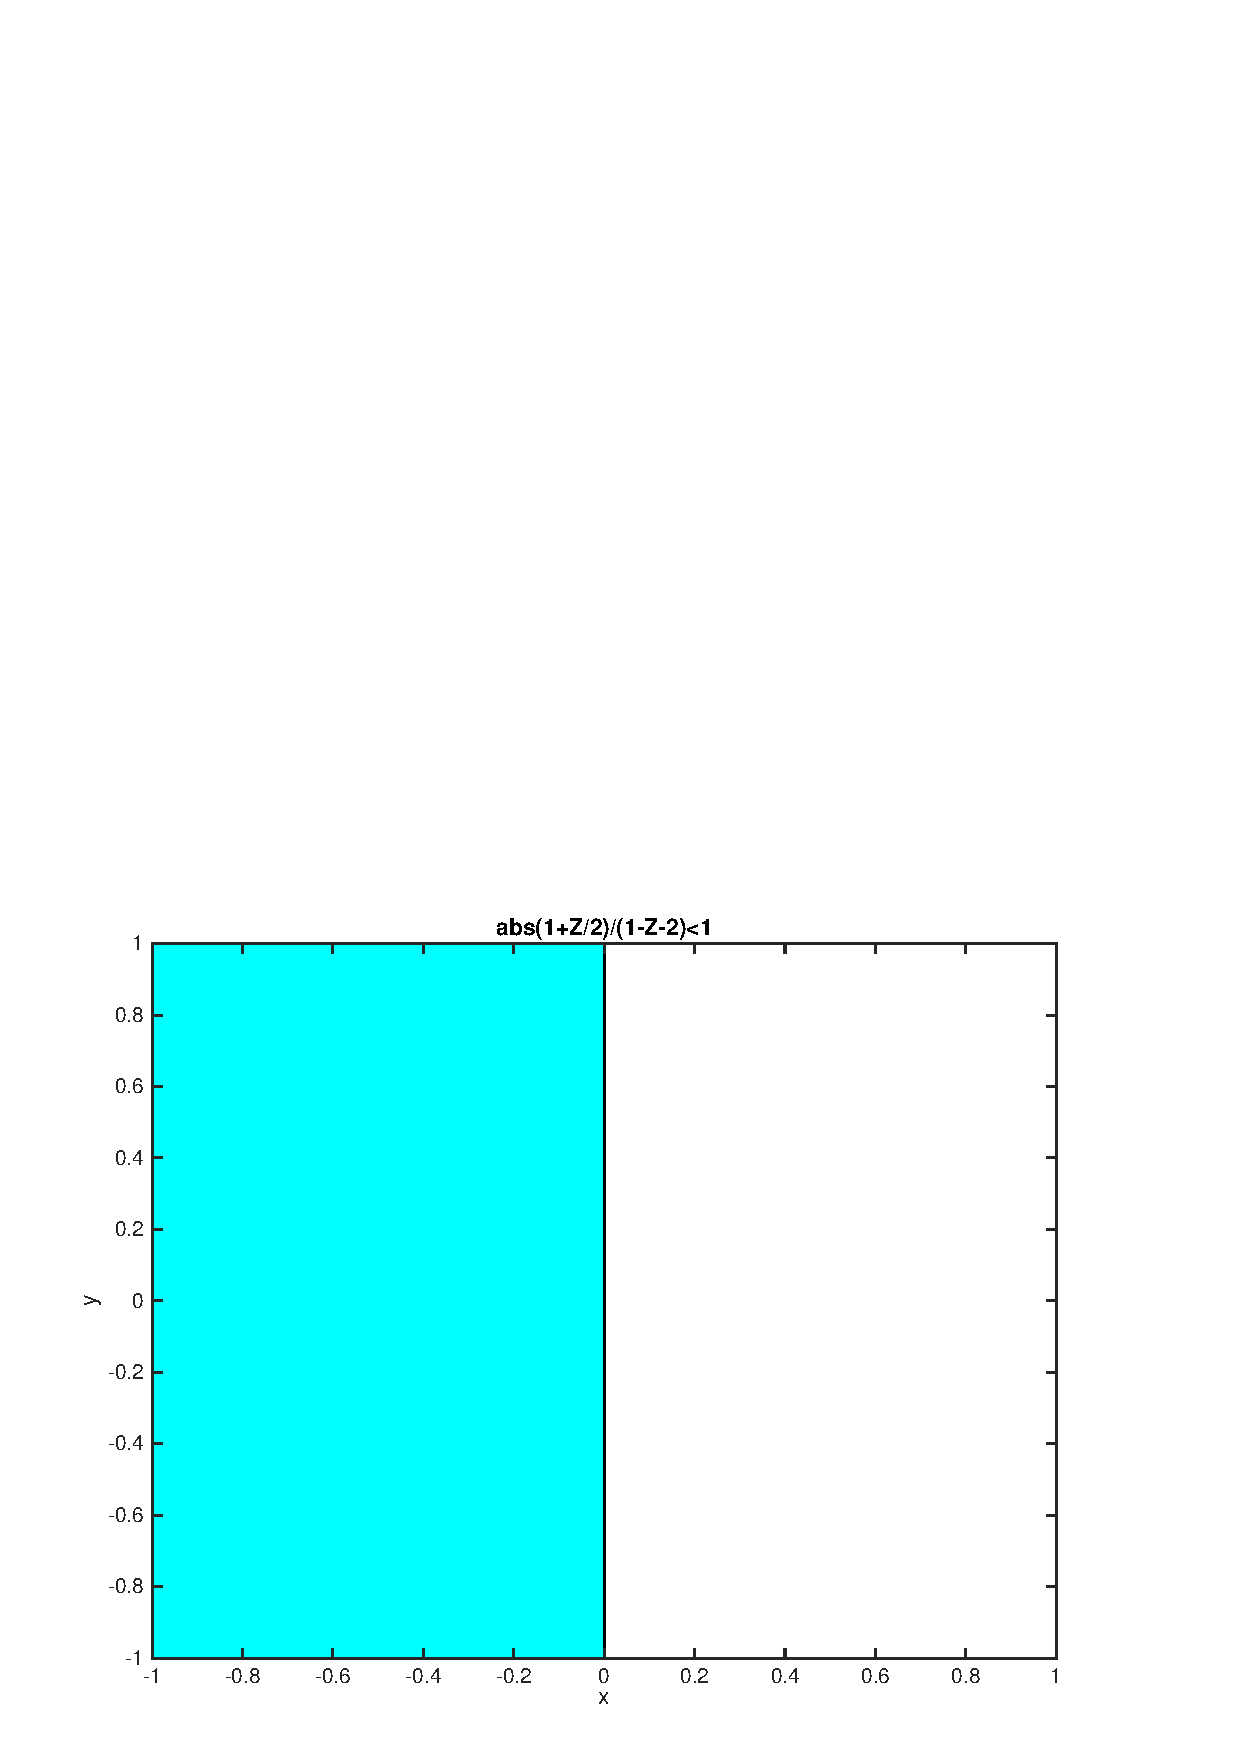
\includegraphics[width=8cm]{5.png}
	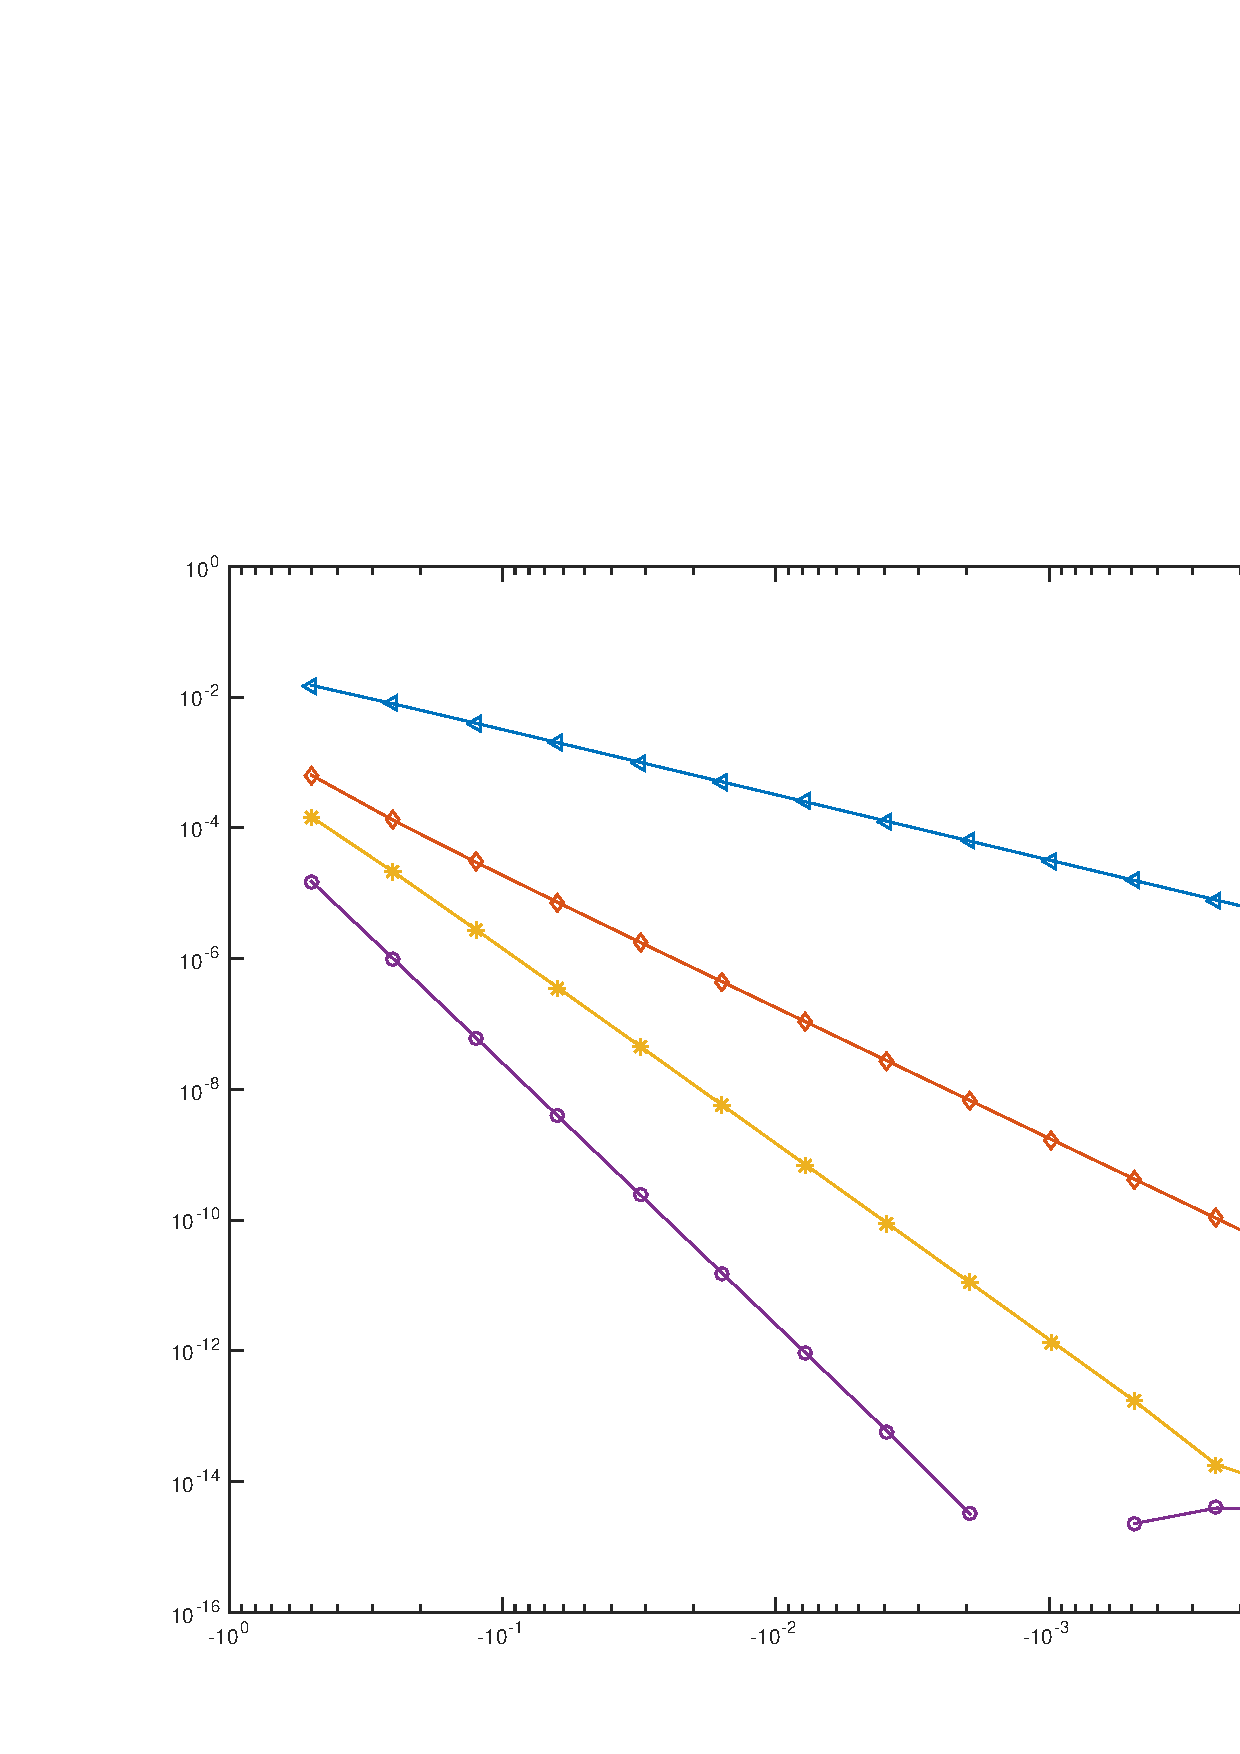
\includegraphics[width=8cm]{6.png}
	\end{center}
	When the noise is added, the peroid of plot of sum is not so clear. In the periodogram plot, periodogram is not always zero in the points outside $\omega$.
	\begin{lstlisting}[language=R,keywordstyle=\color{blue!70},commentstyle=\color{red!50!green!50!blue!50},frame=single, rulesepcolor=\color{red!20!green!20!blue!20},backgroundcolor=\color{backcolour},
]
#Example 4.1
n = 100
x1 = 2*cos(2*pi*1:n*6/100) + 3*sin(2*pi*1:n*6/100)
x2 = 4*cos(2*pi*1:n*10/100) + 5*sin(2*pi*1:n*10/100)
x3 = 6*cos(2*pi*1:n*40/100) + 7*sin(2*pi*1:n*40/100)
x = x1 + x2 + x3 + rnorm(100, sd=5)
par(mfrow=c(2,2))
plot.ts(x1, ylim=c(-10,10), main=expression(omega==6/100~~~A^2==13))
plot.ts(x2, ylim=c(-10,10), main=expression(omega==10/100~~~A^2==41))
plot.ts(x3, ylim=c(-10,10), main=expression(omega==40/100~~~A^2==85))
plot.ts(x, ylim=c(-16,16), main="sum")

#Example 4.2
P = abs(2*fft(x)/100)^2
Fr = 0:(n-1)/100
plot(Fr, P, type='o', xlab="frequency", ylab="periodogram")
	\end{lstlisting}
\item[4.3]
	\begin{align*}
		\mu_x(t)&=\mbe{\suml k1q [U_{k1}\cos(2\pi \omega_kt)+U_{k2}\sin(2\pi\omega_k t)]}\\&=0\\
		\gamma(h)&=\mbe{x_tx_{t+h}}\\
			&=\mbe{\suml k1q [U_{k1}\cos(2\pi \omega_kt)+U_{k2}\sin(2\pi\omega_k t)]\suml k1q [U_{k1}\cos(2\pi \omega_k(t+h))+U_{k2}\sin(2\pi\omega_k (t+h))]}\\
			&=\suml k1q \suml l1q\mbe{[U_{k1}\cos(2\pi \omega_kt)+U_{k2}\sin(2\pi\omega_k t)][U_{l1}\cos(2\pi \omega_k(t+h))+U_{l2}\sin(2\pi\omega_k (t+h))]}\\
			&=\suml k1q \mbe{[U_{k1}\cos(2\pi \omega_kt)+U_{k2}\sin(2\pi\omega_k t)][U_{k1}\cos(2\pi \omega_kt)+U_{k2}\sin(2\pi\omega_k t)]}\\
			&=\suml k1q \sigma_k^2\cos(2\pi\omega_kh)
	\end{align*}
\end{enumerate}

\end{CJK*}
\end{document}
